\section{Inclusive $\pi$ Analysis}\label{sec:PionAnalysis}

In this section we will give an overview of the $\pi^{-}$-inclusive cross-section analysis specific cuts as well as a summary of the ``thin-slice'' method used to extract the inclusive cross-section.


%%%%%%%%%%%%%%%%%%%%%%%%%%%%%%%%%%%%%%%%%%%%%%%%%%%%%%%
\subsection{Overview of Pion TPC Candidate ID}\label{sec:TPCCandidateSelect}
%%%%%%%%%%%%%%%%%%%%%%%%%%%%%%%%%%%%%%%%%%%%%%%%%%%%%%%
Wherever possible, data and Monte Carlo are treated identically for the analysis specific cuts. The selection criteria were developed for this analysis to identify events in which the measured $\pi, \mu, e$ candidate track from the beamline could be matched to activity within the LArTPC. Selections are made to allow disambiguating the activity in the TPC and matching this to the beamline track as well as attempting to reject activity which comes from electromagnetic showers (e.g. electrons and photons) in the beamline.

\begin{itemize}
\item{\textbf{Require the presence of a track in the upstream portion of the TPC}}\\

To select events which can be well matched to the reconstructed WC-track, we require at least one of the TPC reconstructed tracks to have a spacepoint within the first 2 cm in z coordinate, as shown in Fig.\ref{fig:UsFilter0}. An event is rejected if none of the reconstructed tracks have a space point with $0 < z < 2$ cm. The choice of 2~cm distance was arrived at from MC studies outlined in \href{https://lartpc-docdb.fnal.gov:441/cgi-bin/ShowDocument?docid=1766}{docDB-1766} , \href{https://lartpc-docdb.fnal.gov:441/cgi-bin/ShowDocument?docid=1778}{docDB-1778}, \href{https://lartpc-docdb.fnal.gov:441/cgi-bin/ShowDocument?docid=1784}{docDB-1784}

\item{\textbf{Track Multiplicity Requirement}}\\
To reduce both the number of events with high pile-up as well as to reject events which have an electromagnetic shower developing early in the upstream portion of the TPC, we filter events based on the number of tracks present in the region from 0~cm<$z$<14~cm. If more than three tracks are found in this region, the event is removed. The region 0~cm<$z$<14~cm and the requirements of less than four tracks was chosen by comparing pion MC to electron/photon MC as well as looking at a preliminary sample of data (as outlined in \href{https://lartpc-docdb.fnal.gov:441/cgi-bin/ShowDocument?docid=1766}{docDB-1766} , \href{https://lartpc-docdb.fnal.gov:441/cgi-bin/ShowDocument?docid=1778}{docDB-1778}, \href{https://lartpc-docdb.fnal.gov:441/cgi-bin/ShowDocument?docid=1784}{docDB-1784})

\item{\textbf{Shower Rejection}}\\

Hand-scanning a sample of data from Run-I it was found that after applying the selection criteria previously mentioned, there remained a significant sample of residual electromagnetic showers aligned with beam (see Figure \ref{fig:stillShow}). 

\begin{figure}[h!]
\centering
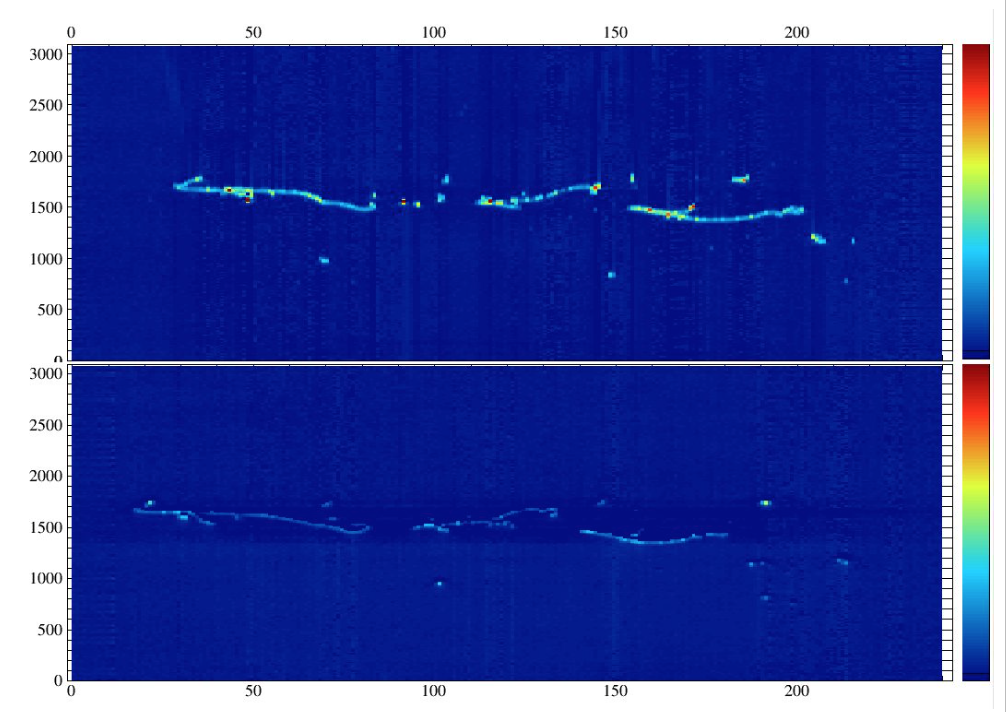
\includegraphics[scale=0.45]{./images/showerEvent.png}
\caption{Example of a "shower-like" event that passes all the previous selection cuts.}
\label{fig:stillShow}
\end{figure}

To eliminate events like this we utilize a simple ``track-based'' filter which, as shown from MC studies, removes a large number of electromagnetic events while still keeping pion events. 

This filter evaluates how many tracks in the TPC are reconstructed for the event and the length for each of these tracks. We then count how many of those tracks would be classified as "short tracks" where ``short'' is any track with length less than 5 cm. Events with more than two ``short'' tracks are removed from consideration. Figure \ref{fig:showrej} shows a graphical representation of this shower based event filter.

\begin{figure}[h!]
\centering
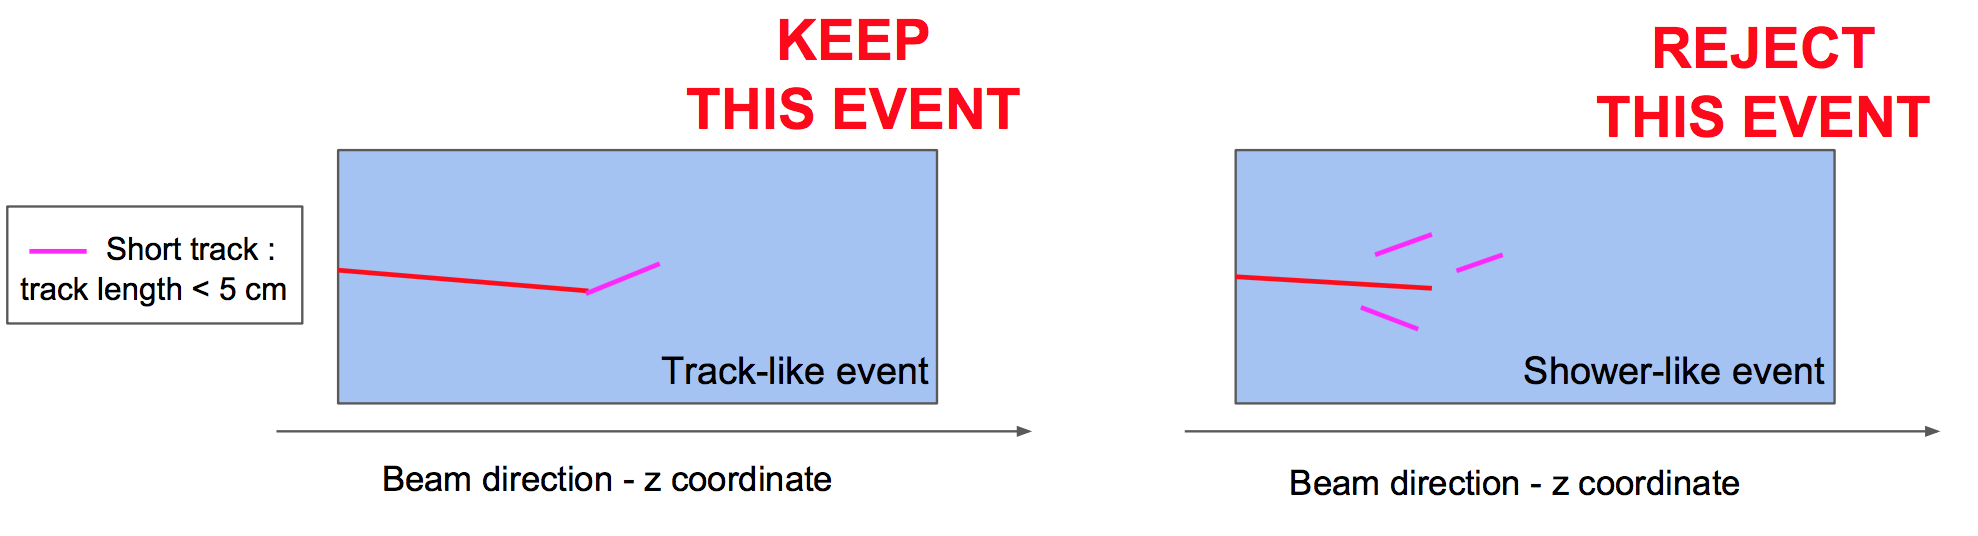
\includegraphics[scale=0.45]{./images/ShowerRejection.png}
\caption{Representation of the Residual Showers Rejection cut.}
\label{fig:showrej}
\end{figure}

The number of ``short'' tracks and the length of the tracks has been chosen utilizing a preliminary scan of the open box data sample and comparing the values to the single particle Monte Carlo attempting to maximize our signal compared to the background.

\item{\textbf{WC to TPC Track Match}}\\

We attempt to uniquely match one WC-Track to one and only one reconstructed TPC track. This match is done to the upstream most point of the TPC track by matching in the $X$ and $Y$ coordinate of the extrapolated WC-Track to the upstream most point of the reconstructed TPC Track as well as matching the incoming track angle to the reconstructed TPC track angle.

We define $\Delta$X as the difference between the $x$ position of the most upstream point of the TPC track and the $x$ position of the WC track as projected to the TPC front face. $\Delta$Y is defined analogously. $\Delta\alpha$ is the angle between the incident WC Track and the TPC track in the plane that contains them. If a Wire Chamber Track to TPC match is found with a  -4~cm~$< \Delta X<$ 6~cm, -5~cm $ < \Delta Y< $~5~cm, and $\alpha < $ 10$^o$ then we consider this a ``well matched'' track. We require each event to have one and only one well matched WC-Track/TPC Track pair.

\begin{figure}[h!]
\centering
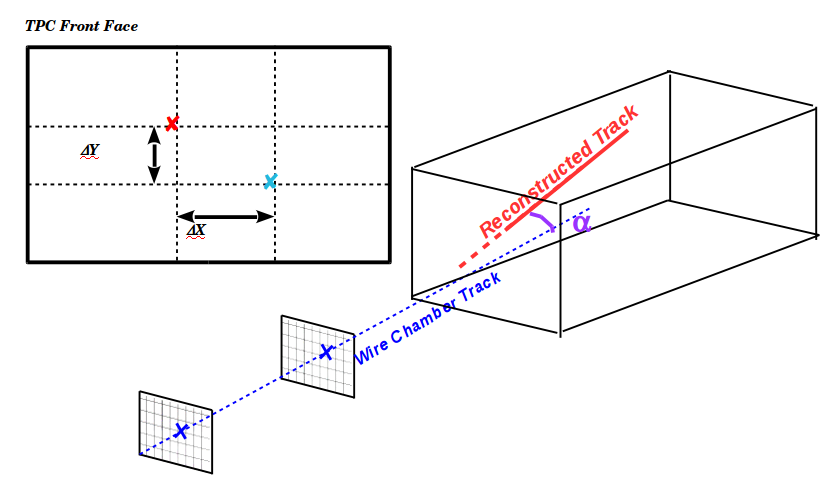
\includegraphics[scale=0.35]{./images/WCTPCMatchSchematic.png}
\caption{Schematic which shows the matching between Wire Chamber tracks and TPC tracks (top) as well as MC particles and TPC tracks.}
\label{fig:WCTrackMatching}
\end{figure}

In the Monte Carlo, there is no reconstructed WC-Track, so instead a projected track from the point of generation is made simulate the WC-Track. The reconstructed MC-track is then matched to this projected point at the front face of the TPC. While this method does not capture the efficiency associated with the wire chamber track algorithm itself, it does allow for a matching based on the data topology and momentum.

\end{itemize}

Having now developed the method by which we select the pion candidate track and have this track uniquely matched to a wire chamber track, we can proceed with analyzing this to establish the cross-section. In order to do this, it is necessary to lay out the general technique used in this analysis.

%%%%%%%%%%%%%%%%%%%%%%%%%%%%%%%%%%%%%%%%%%%%%%%%%%%%%%%%%
\subsection{Thin slice method}\label{sec:ThinSlice}
%%%%%%%%%%%%%%%%%%%%%%%%%%%%%%%%%%%%%%%%%%%%%%%%%%%%%%%%%
In general, the target is not a single particle, but a slab of material containing many diffusion centers. If we assume the target centers to be uniformly distributed in the material and the target to be thin enough not to have one center sitting in front of another, we are in the so-called  "thin target" approximation. A pictorial representation of the ``thin slice'' approximation is shown schematically in Figure \ref{fig:thinslice}


\begin{figure}[htb]
\centering
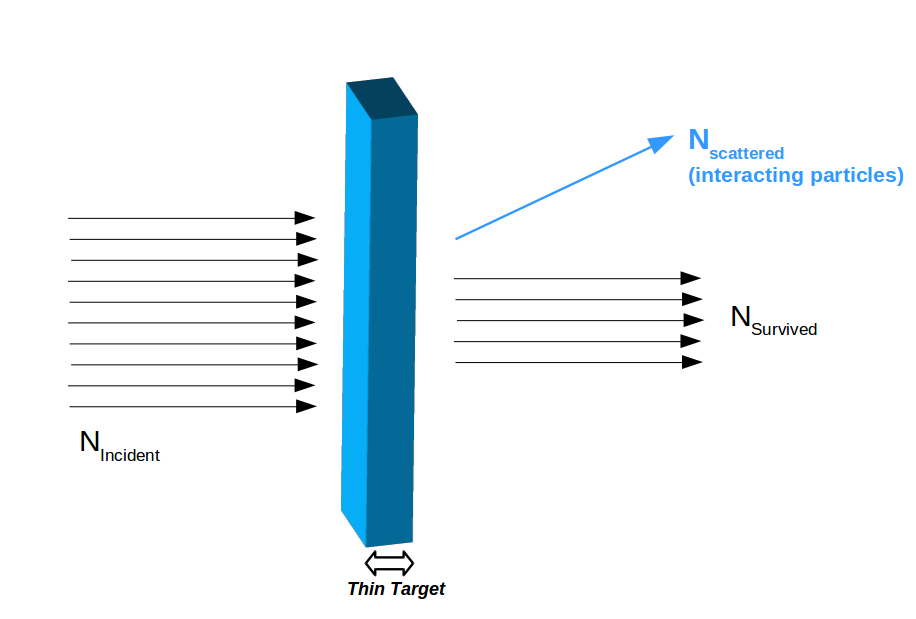
\includegraphics[scale=0.25]{./images/ThinTarget.png}
\caption{Representation of the thin target approximation as a ``thin slice'' of argon.}
\label{fig:thinslice}
\end{figure}

The survival probability of a pion traveling through a slab of argon of depth {\it z} and density {\it n} is given by

\begin{equation}
P_{survival} = e^{-\sigma_{total}n z},
\end{equation} 

where $\sigma_{tot}$ is the total cross section per nucleon (in $cm^2$). Then the interaction probability is given by one minus the survial probability
\begin{equation}
P_{interacting} = 1 - P_{survial}.
\end{equation}
Experimentally we can measure interaction probability ($P_{interacting}$) by measuring the ratio of the number of interacting pions to the number of incident pions, $N_{interacting}/N_{incident}$ for a given slab at a given energy:

\begin{equation}\label{eqn:ProbInteraction}
P_{interacting}=\frac{N_{interacting}}{N_{incident}}=1-e^{-\sigma_{tot}n z}
\end{equation}

By expanding Equation \ref{eqn:ProbInteraction} (assuming a small $z$ slab) the probability of interacting can be expressed as

\begin{equation}
P_{interacting} = 1 - (1-\sigma_{total}n z \delta + ...).
\end{equation}

Rearranging this expression, the measured rate of interactions can be used to calculate the total cross section as a function of energy
\begin{equation}\label{calc_sigma}
\sigma_{tot}(E) \simeq \frac{1}{nz} \Big(\frac{N_{interacting}}{N_{incident}}\Big) 
\end{equation}
where {\emph{z}} is the target thickness (in cm) along the incident pion direction, and {\emph{n}} is the scattering center density in the target, $n=\frac{\rho N_{A} }{A}$ (in $cm^{-3}$). 

The uncertainty for each energy bin is calculated by error propagation from the uncertainty on $N_{incident}$ and $N_{interacting}$. 
Since the number of incident pions in each slice is given by a simple counting, it is safe to assume that $N_{incident}$ is distributed as a poissonian with mean and $\sigma^2$ equal to $N_{incident}$ in each bin.  
On the other hand, $N_{interacting}$ follows a binomial distribution: the particle in a given energy bin might or might not interact.  The interaction probability $p$ is $\frac{ N_{interacting}}{N_{incident}}$ and the number of tries $n$ is $N_{incident}$. 
So, the square of the variance for the binomial is given by  $$\sigma^2 = np(1-p) =  N_{incident}\frac{ N_{interacting}}{N_{incident}} (1-\frac{ N_{interacting}}{N_{incident}}) = N_{interacting}(1-\frac{ N_{interacting}}{N_{incident}}).$$

$N_{incident}$ and $N_{interacting}$ are not independent.
The uncertainty on the cross section is thus calculated as 
\begin{equation}
\delta\sigma_{tot}(E) = \sigma_{tot}(E) \Big(\frac{\delta N_{interacting}}{N_{interacting}}+\frac{\delta N_{incident}}{N_{incident}}\Big) 
\end{equation}
where:
\begin{eqnarray}
\delta N_{incident} = \sqrt[]{N_{incident}} \\
\delta N_{interacting} = \sqrt[]{N_{interacting}(1-\frac{ N_{interacting}}{N_{incident}})}.
\end{eqnarray}

%%%%%%%%%%%%%%%%%%%%%%%%%%%%%%%%%%%%%%%%%%%%%%%%%%%%%%%%%%%%%%%%%%%%%%%%%%
\subsection{Thick Target Method - Slicing the LArTPC in thin targets}
%%%%%%%%%%%%%%%%%%%%%%%%%%%%%%%%%%%%%%%%%%%%%%%%%%%%%%%%%%%%%%%%%%%%%%%%%% 

When the "thin target" approach is not applicable, such as in the case of "thick target" experiments like LArIAT, a slightly different technique is needed in order to accurately evaluate the pion cross section dependence on energy. In particular, one must know the energy loss of the pion as it crosses the "thick" target before reaching its interaction point. In the ``thin slice'' approximation it is reasonable to only consider the $\pi$-nucleus hadronic interactions, while for the "thick" target case, it is necessary to take into account other pion interactions such as pion decay (both in flight and at rest) as well as pion capture at rest on the target nuclei.

A new technique, called the "sliced TPC" method, was developed in order to make the measurement possible in the thick target LArTPC~\cite{myThesis} environment. The fine-grained tracking of the LArIAT LArTPC allows us to treat the 90-cm thick LAr volume as a sequence of many adjacent thin targets. 

For LArIAT, the two wire planes are each composed of 240 wires oriented at +/- $60^{\circ}$ at 4 mm spacing. The wires collect signals proportional to the energy loss of the pion in a $60^{\circ}$-inclined 4~mm thin slab of liquid argon. Thus, one can think of the TPC as being subdivided into many slices of $\Delta${\emph{z}} = 4 mm/sin($60^{\circ}$) $\approx$ 4.5~mm thickness along the {\emph{z}} axis, i.e., direction of the incident particles (pions), as shown in Fig.~\ref{fig:slicedtpc}. 

Each slice {\emph{n}} can be now considered as a "thin target" and we can apply the cross section calculation from Eq.~\ref{calc_sigma} iteratively, evaluating the actual kinetic energy of the pion as it enters each slice, $E_{n}^{kin}$. The energy of the pion entering the TPC is known by the momentum determination of the tertiary beamline, and the incident energy of the pion at the successive slab is determined by subtraction of the calorimetric energy released by the particle in the previous slab. If the particle enters a slice, it contributes to $N_{incident}$ in the energy bin corresponding to its kinetic energy in that slice. If it interacts in the slice, it then also contributes to $N_{interacting}$ in the appropriate energy bin.

%\textcolor{blue}{Sketch of sliced tpc technique?}
\begin{figure}[ht!]
\centering
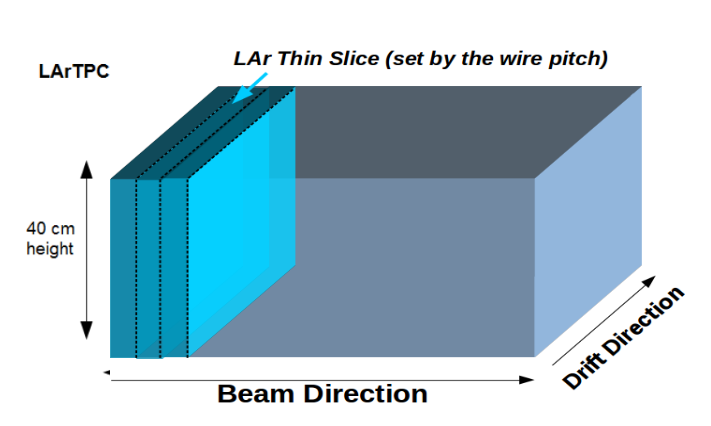
\includegraphics[scale=0.35]{./images/SlicedTPC.png}\\
\caption{Sketch of Sliced TPC approach.}
\label{fig:slicedtpc}
\end{figure}

The "sliced TPC" technique was tested by comparing the results of this method with the prediction of the total hadronic interaction cross section ($\pi^{\pm}$, Ar) for thin-target simulations from two Monte Carlo generators (Geant 4.10.1 with Bertini Cascade model~\cite{geant4, g4bert} and Genie v2.8.2 with intranuke-hA model). The thick target simulation used a simple stand-alone Geant4 simulation  (i.e., no other detector features were taken into account except the geometry of the thin slices in the LAr volume). Fig.~\ref{fig:xsplot} shows the resulting total ${\pi^-}$ cross section extracted by the sliced TPC technique; it agrees well with the Geant 4 thin-target cross section. The Genie thin-target cross section for $^{40}$Ar shown in this figure is significantly different than that of Geant at low kinetic energies due to the fact that Geant4 models are tuned on $^{12}$C while Genie ones are tuned on a much heavier $^{56}$Fe target. The extrapolated cross section predicted for $^{40}$Ar can be then very different, especially in the resonance region where the model is strongly target-dependent from one generator to another.
 
The comparison of the Geant4 thin- and thick-target cross section results demonstrates the power of the "sliced TPC" method for the measurement of the ($\pi^{\pm}$, Ar) cross section in LArIAT TPC geometry. 

\begin{figure}[h!]
\centering
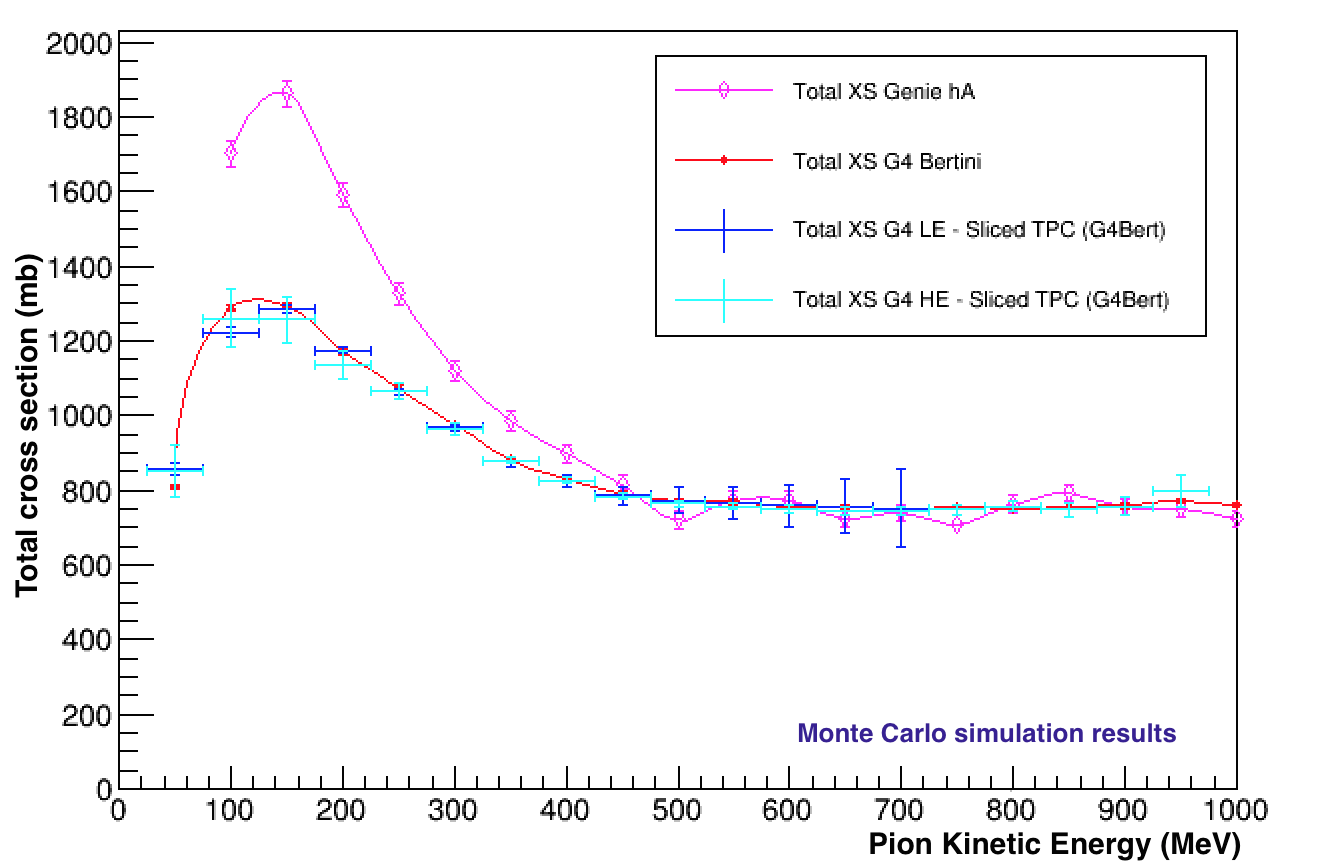
\includegraphics[scale=0.45]{./images/compare_new.png}
\caption{$\pi^-$ on Ar total cross section dependence on the kinetic energy from MC simulations: comparison between Geant4 and Genie predictions for a LAr thin target and extrapolated cross section with the ``Sliced TPC'' approach with a Geant4 Bertini based simulation of the LArTPC thick target \cite{myThesis}.}
\label{fig:xsplot}
\end{figure}

Having validated the ``Sliced TPC'' technique and shown that the this technique recovers the simulated cross-section, we now move to performing this measurement utilizing the complete LArIAT simulation within the LArSoft \cite{} based simulation.  Furthermore, we move from utilizing particle level MC-truth information to performing fully automated reconstruction of the charged pion events within the LArTPC. 



